\documentclass[aspectratio=169]{beamer}

\usetheme{Madrid}
\usecolortheme{default}
\usepackage{booktabs}
\usepackage{graphicx}
\usepackage{adjustbox}
\usepackage{xcolor}
\usepackage{tikz}
\usepackage{multirow}

% Custom colors
\definecolor{bestcolor}{RGB}{0,100,0}

% Bold + color helper for best scores
\newcommand{\best}[1]{\textcolor{bestcolor}{\textbf{#1}}}

\title[Progress Report]{Comparative Analysis of Transformer Architectures\\for Multilingual News Classification}
\subtitle{Progress Recording -- Experiment Results Update}
\author{Experiment Team}
\institute{Supervised Fine-Tuning with LoRA Adapters}
\date{\today}

\begin{document}

% ============================================================
% Slide 1: Title
% ============================================================
\begin{frame}
  \titlepage
\end{frame}

% ============================================================
% Slide 2: Outline
% ============================================================
\begin{frame}{Outline}
  \tableofcontents
\end{frame}

% ============================================================
\section{Introduction}
% ============================================================

% Slide 3: Project Overview
\begin{frame}{Project Overview}
  \begin{block}{Research Goal}
    Compare transformer encoder architectures on \textbf{multilingual} political
    and fake news classification using \textbf{LoRA} (Low-Rank Adaptation)
    parameter-efficient fine-tuning.
  \end{block}

  \vspace{0.3cm}
  \textbf{Key aspects:}
  \begin{itemize}
    \item Four encoder models evaluated across \textbf{8 datasets} in \textbf{3 languages} (English, Bulgarian, Arabic)
    \item Task types: binary classification (hyperpartisan, fake news, harmful tweet detection) and multi-class classification (political leaning, propaganda detection)
    \item Metrics: \textbf{Accuracy} and \textbf{Weighted F1-Score}
    \item Each experiment averaged over \textbf{5 runs} for reliability
  \end{itemize}
\end{frame}

% ============================================================
\section{Datasets}
% ============================================================

% Slide 4: Datasets Overview
\begin{frame}{Datasets Overview}
  \begin{table}
    \centering
    \scriptsize
    \begin{adjustbox}{max width=\textwidth}
    \begin{tabular}{llcccc}
      \toprule
      \textbf{Dataset} & \textbf{Task} & \textbf{Language} & \textbf{Classes} & \textbf{Approx.\ Size} & \textbf{Labels} \\
      \midrule
      Hyperpartisan News Headlines & Hyperpartisan detection & English    & 2 & 2,200   & neutral / hyperpartisan \\
      SemEval 2019                 & Hyperpartisan detection & English    & 2 & 1,275   & neutral / hyperpartisan \\
      All Sides                    & Political leaning       & English    & 3 & 45,411  & left / center / right \\
      Fake News Net                & Fake news detection     & English    & 2 & 23,200  & true / fake \\
      CLEF 3A                      & Propaganda detection    & English    & 3 & 206,373 & multi-level propaganda \\
      \midrule
      CLEF 1C (en)                 & Harmful tweet detection & English    & 2 & 3,574   & neutral / harmful \\
      CLEF 1C (bg)                 & Harmful tweet detection & Bulgarian  & 2 & 3,033   & neutral / harmful \\
      CLEF 1C (ar)                 & Harmful tweet detection & Arabic     & 2 & 4,825   & neutral / harmful \\
      \bottomrule
    \end{tabular}
    \end{adjustbox}
  \end{table}

  \vspace{0.15cm}
  \begin{itemize}
    \item \textbf{5 English} news/article datasets + \textbf{3 multilingual} CLEF 1C tweet datasets (en/bg/ar).
    \item CLEF 1C datasets are \textbf{highly imbalanced}: 77--91\% neutral class.
  \end{itemize}
\end{frame}

% ============================================================
\section{Experiment Setup}
% ============================================================

% Slide 5: Models & LoRA Configuration
\begin{frame}{Models \& LoRA Configuration}
  \begin{columns}[T]
    \begin{column}{0.48\textwidth}
      \textbf{Encoder Models Evaluated:}
      \begin{enumerate}
        \item \texttt{FacebookAI/roberta-base}
        \item \texttt{FacebookAI/roberta-large}
        \item \texttt{answerdotai/ModernBERT-base}
        \item \texttt{launch/POLITICS}
      \end{enumerate}
      \vspace{0.3cm}
      \small
      \textit{POLITICS} is a domain-specific model pre-trained on political news corpora.
    \end{column}
    \begin{column}{0.48\textwidth}
      \textbf{LoRA Configuration:}
      \begin{table}
        \small
        \begin{tabular}{ll}
          \toprule
          \textbf{Parameter} & \textbf{Value} \\
          \midrule
          Rank ($r$)         & 8 \\
          Alpha ($\alpha$)   & 16 \\
          Dropout            & 0.1 \\
          Bias               & none \\
          Task type          & SEQ\_CLS \\
          \bottomrule
        \end{tabular}
      \end{table}
    \end{column}
  \end{columns}
\end{frame}

% Slide 6: Training Hyperparameters
\begin{frame}{Training Hyperparameters}
  \begin{columns}[T]
    \begin{column}{0.48\textwidth}
      \begin{table}
        \small
        \begin{tabular}{ll}
          \toprule
          \textbf{Hyperparameter} & \textbf{Value} \\
          \midrule
          Epochs             & 3 \\
          Batch size         & 8 \\
          Learning rate      & $1 \times 10^{-4}$ \\
          LR scheduler       & Constant \\
          Warmup ratio       & 0.1 \\
          Max grad norm      & 0.3 \\
          Weight decay       & 0.001 \\
          Max seq.\ length   & 512 \\
          FP16               & Enabled \\
          Runs               & 5 \\
          \bottomrule
        \end{tabular}
      \end{table}
    \end{column}
    \begin{column}{0.48\textwidth}
      \textbf{Evaluation Protocol:}
      \begin{itemize}
        \item Evaluation at the end of each epoch
        \item 10\% of training data held out for validation
        \item Final metrics computed on the \textbf{test set}
        \item Results averaged over \textbf{5 independent runs}
        \item Weighted averaging for precision, recall, and F1
      \end{itemize}
      \vspace{0.3cm}
      \textbf{Hardware:} Single NVIDIA A40 (30\,GB)
    \end{column}
  \end{columns}
\end{frame}

% ============================================================
\section{Experiment Results}
% ============================================================

% Slide 7: Full Results Table
\begin{frame}{Experiment Results -- Full Table}
  \begin{table}
    \centering
    \scriptsize
    \begin{adjustbox}{max width=\textwidth}
    \begin{tabular}{llcccccccc}
      \toprule
      \textbf{Model} & \textbf{Metric}
        & \textbf{Hyperpartisan} & \textbf{SemEval}
        & \textbf{All Sides} & \textbf{FakeNewsNet}
        & \textbf{CLEF 3A}
        & \textbf{CLEF 1C\_en} & \textbf{CLEF 1C\_bg} & \textbf{CLEF 1C\_ar} \\
      \midrule
      \multirow{2}{*}{roberta-base}
        & Acc & 0.7950          & \best{0.8684} & 0.6524          & 0.8574          & 0.7106          & 0.7277          & \best{0.9661} & \best{0.8351} \\
        & F1  & 0.7905          & \best{0.8676} & 0.6434          & 0.8464          & 0.7184          & 0.7572          & \best{0.9495} & 0.7815 \\
      \midrule
      \multirow{2}{*}{roberta-large}
        & Acc & \best{0.8593}   & 0.8556        & \best{0.7139}   & \best{0.8644}   & \best{0.7546}   & 0.7636          & \best{0.9661} & 0.8312 \\
        & F1  & \best{0.8552}   & 0.8549        & \best{0.7057}   & \best{0.8548}   & \best{0.7585}   & \best{0.7909}   & \best{0.9495} & 0.7935 \\
      \midrule
      \multirow{2}{*}{ModernBERT-base}
        & Acc & 0.7538          & 0.8009        & 0.6046          & 0.8528          & 0.6342          & 0.7184          & 0.9495        & 0.8087 \\
        & F1  & 0.7302          & 0.8006        & 0.5901          & 0.8413          & 0.6364          & 0.7457          & \best{0.9495} & \best{0.8087} \\
      \midrule
      \multirow{2}{*}{POLITICS}
        & Acc & 0.8358          & 0.8444        & 0.6937          & 0.8586          & 0.7160          & \best{0.7662}   & \best{0.9661} & 0.8281 \\
        & F1  & 0.8333          & 0.8435        & 0.6852          & 0.8505          & 0.7201          & 0.7825          & \best{0.9495} & 0.8055 \\
      \bottomrule
    \end{tabular}
    \end{adjustbox}
  \end{table}

  \vspace{0.1cm}
  \centering
  \scriptsize
  \textcolor{bestcolor}{\textbf{Bold green}} = best score per dataset column. All results averaged over 5 runs.
\end{frame}

% Slide 8: Multilingual CLEF 1C Spotlight
\begin{frame}{Spotlight: Multilingual CLEF 1C Results}
  \begin{columns}[T]
    \begin{column}{0.55\textwidth}
      \begin{table}
        \centering
        \small
        \begin{adjustbox}{max width=\textwidth}
        \begin{tabular}{llccc}
          \toprule
          \textbf{Model} & \textbf{Metric}
            & \textbf{English} & \textbf{Bulgarian} & \textbf{Arabic} \\
          \midrule
          \multirow{2}{*}{roberta-base}
            & Acc & 0.7277          & \best{0.9661} & \best{0.8351} \\
            & F1  & 0.7572          & \best{0.9495} & 0.7815 \\
          \midrule
          \multirow{2}{*}{roberta-large}
            & Acc & 0.7636          & \best{0.9661} & 0.8312 \\
            & F1  & \best{0.7909}   & \best{0.9495} & 0.7935 \\
          \midrule
          \multirow{2}{*}{ModernBERT}
            & Acc & 0.7184          & 0.9495        & 0.8087 \\
            & F1  & 0.7457          & \best{0.9495} & \best{0.8087} \\
          \midrule
          \multirow{2}{*}{POLITICS}
            & Acc & \best{0.7662}   & \best{0.9661} & 0.8281 \\
            & F1  & 0.7825          & \best{0.9495} & 0.8055 \\
          \bottomrule
        \end{tabular}
        \end{adjustbox}
      \end{table}
    \end{column}
    \begin{column}{0.42\textwidth}
      \textbf{Key observations:}
      \begin{itemize}
        \item \textbf{Bulgarian} is nearly solved: all models $\geq$0.95 F1 (heavily imbalanced toward neutral)
        \item \textbf{Arabic}: ModernBERT achieves best F1 (0.809) despite trailing on English tasks
        \item \textbf{English} is the hardest CLEF 1C split; POLITICS leads in Acc
        \item English-only models perform surprisingly well on non-English tweets
      \end{itemize}
    \end{column}
  \end{columns}
\end{frame}

% ============================================================
\section{Key Findings}
% ============================================================

% Slide 9: Key Findings (1)
\begin{frame}{Key Findings (1/2)}
  \begin{block}{1.\ RoBERTa-large is the overall best model}
    Achieves the highest scores on \textbf{5+ out of 8} datasets across metrics. Scaling from base to large yields consistent improvements of \textbf{+3--6\%} on English tasks.
  \end{block}

  \begin{block}{2.\ POLITICS benefits from domain-specific pre-training}
    Despite being a base-sized model, ranks \textbf{2nd overall} and narrows the gap with roberta-large on political tasks:
    \begin{itemize}
      \item All Sides: 0.694 Acc vs.\ roberta-base's 0.652 (\textbf{+4.1\%})
      \item CLEF 1C (en): best accuracy at 0.766, outperforming roberta-large's 0.764
    \end{itemize}
  \end{block}

  \begin{block}{3.\ SemEval 2019 anomaly: smaller model wins}
    RoBERTa-base \textbf{outperforms} roberta-large (0.868 vs.\ 0.856 Acc). The small dataset ($\sim$1.3K) likely causes the larger model to overfit.
  \end{block}
\end{frame}

% Slide 10: Key Findings (2)
\begin{frame}{Key Findings (2/2)}
  \begin{block}{4.\ English-only models transfer surprisingly well to non-English tasks}
    On CLEF 1C Bulgarian, all models achieve $\geq$0.95 F1. On Arabic, roberta-base leads with 0.835 Acc. This suggests English-centric models can exploit \textbf{structural and lexical overlap} in tweet-level classification.
  \end{block}

  \begin{block}{5.\ ModernBERT shows strength on Arabic despite overall weakness}
    While ModernBERT-base underperforms on most English tasks, it achieves the \textbf{best F1 on Arabic} CLEF 1C (0.809), suggesting its architecture may handle certain cross-lingual patterns better.
  \end{block}

  \begin{block}{6.\ Task and class complexity dominate difficulty}
    Multi-class tasks (All Sides, CLEF 3A) remain the hardest. CLEF 1C Bulgarian appears easiest due to extreme class imbalance ($\sim$87\% neutral) -- high scores may reflect majority-class bias.
  \end{block}
\end{frame}

% ============================================================
\section{Future Work}
% ============================================================

% Slide 11: Future Work
\begin{frame}{Future Work \& Potential Improvements}
  \begin{columns}[T]
    \begin{column}{0.48\textwidth}
      \textbf{Expand Model Coverage:}
      \begin{itemize}
        \item Add \textbf{decoder models}: Llama-3.1-8B, Mistral-Nemo, Qwen2.5-7B with LoRA SFT
        \item Compare encoder SFT vs.\ decoder SFT
        \item Evaluate \textbf{in-context learning}: zero-shot, chain-of-thought, and few-shot prompting
      \end{itemize}

      \vspace{0.3cm}
      \textbf{Multilingual Extensions:}
      \begin{itemize}
        \item Add dedicated multilingual encoders: XLM-RoBERTa, mDeBERTa
        \item Evaluate on remaining languages: Portuguese (Fake.br), Spanish (FakeNewsCorpus)
      \end{itemize}
    \end{column}
    \begin{column}{0.48\textwidth}
      \textbf{Methodological Improvements:}
      \begin{itemize}
        \item Hyperparameter search for LoRA rank, alpha, and target modules (especially for ModernBERT)
        \item Report confidence intervals / standard deviations
        \item Class-balanced evaluation metrics for imbalanced CLEF 1C datasets
      \end{itemize}

      \vspace{0.3cm}
      \textbf{Deeper Analysis:}
      \begin{itemize}
        \item Confusion matrices for multi-class and imbalanced tasks
        \item Cross-lingual transfer analysis: why do English models work on bg/ar?
        \item Computational cost comparison
      \end{itemize}
    \end{column}
  \end{columns}
\end{frame}

% ============================================================
% Slide 12: Summary
% ============================================================
\begin{frame}{Summary}
  \begin{center}
    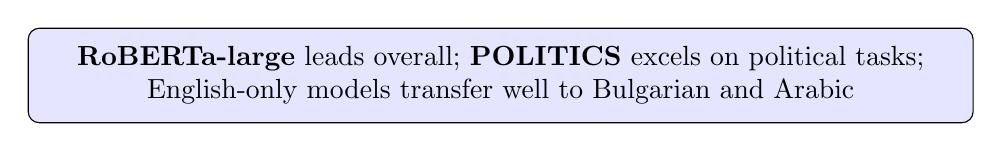
\begin{tikzpicture}
      \node[draw, rounded corners, fill=blue!10, minimum width=12cm, minimum height=1.2cm, text width=11.5cm, align=center] {
        \textbf{RoBERTa-large} leads overall; \textbf{POLITICS} excels on political tasks;\\
        English-only models transfer well to Bulgarian and Arabic
      };
    \end{tikzpicture}
  \end{center}

  \vspace{0.2cm}
  \textbf{Completed:}
  \begin{itemize}
    \item[\checkmark] Benchmarked 4 encoder models on \textbf{8 datasets} across \textbf{3 languages}
    \item[\checkmark] Established LoRA fine-tuning baselines with 5-run averages
    \item[\checkmark] Identified scaling, domain pre-training, cross-lingual transfer, and task complexity effects
  \end{itemize}

  \vspace{0.2cm}
  \textbf{Next Steps:}
  \begin{itemize}
    \item[$\rightarrow$] Decoder model evaluation and in-context learning experiments
    \item[$\rightarrow$] Dedicated multilingual models (XLM-RoBERTa, mDeBERTa) for non-English tasks
    \item[$\rightarrow$] Class-balanced metrics and deeper cross-lingual transfer analysis
  \end{itemize}
\end{frame}

\end{document}
